%
% "The UCD CASL SenseTile System", for IEEE Pervasive Computing Joseph
% R. Kiniry, Vieri del Bianco, Dragan Stosic $Id: paper.tex 2795
% 2007-09-23 19:35:53Z dmz
%

\documentclass{article} \usepackage{times}

\usepackage{ifpdf} \usepackage{a4wide} \usepackage{pdfsync}

\ifpdf \usepackage[pdftex]{graphicx} \else \usepackage{graphicx} \fi

\usepackage{xspace} \usepackage{tabularx} \usepackage{epsfig}
\usepackage{amsmath} \usepackage{amsfonts} \usepackage{amssymb}
\usepackage{eucal} \usepackage{stmaryrd} \usepackage{float}
\usepackage{listings} % @(#)$Id: jml-listings.tex,v 1.6 2007/06/25 22:37:23 leavens Exp $
%
% Copyright (C) 2006 Iowa State University
%
% This file is part of JML
%
% JML is free software; you can redistribute it and/or modify
% it under the terms of the GNU General Public License as published by
% the Free Software Foundation; either version 2, or (at your option)
% any later version.
%
% JML is distributed in the hope that it will be useful,
% but WITHOUT ANY WARRANTY; without even the implied warranty of
% MERCHANTABILITY or FITNESS FOR A PARTICULAR PURPOSE.  See the
% GNU General Public License for more details.
%
% You should have received a copy of the GNU General Public License
% along with JML; see the file COPYING.  If not, write to
% the Free Software Foundation, 675 Mass Ave, Cambridge, MA 02139, USA.
%
% A JML listings environment.
%
% AUTHOR: Gary T. Leavens
%
% requires listings i.e., do \usepackage{listings} first
%
% This file is set up to be used via % @(#)$Id: jml-listings.tex,v 1.6 2007/06/25 22:37:23 leavens Exp $
%
% Copyright (C) 2006 Iowa State University
%
% This file is part of JML
%
% JML is free software; you can redistribute it and/or modify
% it under the terms of the GNU General Public License as published by
% the Free Software Foundation; either version 2, or (at your option)
% any later version.
%
% JML is distributed in the hope that it will be useful,
% but WITHOUT ANY WARRANTY; without even the implied warranty of
% MERCHANTABILITY or FITNESS FOR A PARTICULAR PURPOSE.  See the
% GNU General Public License for more details.
%
% You should have received a copy of the GNU General Public License
% along with JML; see the file COPYING.  If not, write to
% the Free Software Foundation, 675 Mass Ave, Cambridge, MA 02139, USA.
%
% A JML listings environment.
%
% AUTHOR: Gary T. Leavens
%
% requires listings i.e., do \usepackage{listings} first
%
% This file is set up to be used via % @(#)$Id: jml-listings.tex,v 1.6 2007/06/25 22:37:23 leavens Exp $
%
% Copyright (C) 2006 Iowa State University
%
% This file is part of JML
%
% JML is free software; you can redistribute it and/or modify
% it under the terms of the GNU General Public License as published by
% the Free Software Foundation; either version 2, or (at your option)
% any later version.
%
% JML is distributed in the hope that it will be useful,
% but WITHOUT ANY WARRANTY; without even the implied warranty of
% MERCHANTABILITY or FITNESS FOR A PARTICULAR PURPOSE.  See the
% GNU General Public License for more details.
%
% You should have received a copy of the GNU General Public License
% along with JML; see the file COPYING.  If not, write to
% the Free Software Foundation, 675 Mass Ave, Cambridge, MA 02139, USA.
%
% A JML listings environment.
%
% AUTHOR: Gary T. Leavens
%
% requires listings i.e., do \usepackage{listings} first
%
% This file is set up to be used via \input{jml-listings}.
% If you want, you could make a version that is a style file,
% but then change \lstdefinelanguage to \lst@definelanguage below.
%
\lstdefinelanguage[JML]{Java}[]{Java}%
       {% C++ style comments have to start with a blank!
        comment=[l]{//\ },
        % And C-style comments must also start with a blank or star!
        morecomment=[s]{/*\ }{*/},        
        morecomment=[s]{/**}{*/},
        % sensitive=true, % inherited
        % Add JML keywords as level 1 keywords, so can typeset differently
        classoffset=1,
        % And here are all the wonderful JML keywords
        morekeywords={abrupt_behavior,abrupt_behaviour,
         accessible,accessible_redundantly,also,assert,assert_redundantly,
         assignable,assignable_redundantly,assume,assume_redundantly,
         axiom,behavior,behaviour,breaks,breaks_redundantly,
         callable,callable_redundantly,captures,captures_redundantly,
         choose,choose_if,code,code_bigint_math,code_java_math,
         code_safe_math,constraint,constraint_redundantly,constructor,
         continues,continues_redundantly,decreases,decreases_redundantly,
         decreasing,decreasing_redundantly,diverges,diverges_redundantly,
         duration,duration_redundantly,ensures,ensures_redundantly,
         example,exceptional_behavior,exceptional_behaviour,
         exceptional_example,exsures,exsures_redundantly,extract,field,
         forall,for_example,ghost,helper,hence_by,hence_by_redundantly,
         implies_that,in,in_redundantly,initializer,initially,instance,
         invariant,invariant_redundantly,loop_invariant,
         loop_invariant_redundantly,maintaining,maintaining_redundantly,
         maps,maps_redundantly,measured_by,measured_by_redundantly,method,
         model,model_program,modifiable,modifiable_redundantly,modifies,
         modifies_redundantly,monitored,monitors_for,non_null,
         normal_behavior,normal_behaviour,normal_example,nowarn,
         nullable,nullable_by_default,old,or,post,post_redundantly,
         pre,pre_redundantly,pure,readable,refine,refines,refining,represents,
         represents_redundantly,requires,requires_redundantly,
         returns,returns_redundantly,set,signals,signals_only,
         signals_only_redundantly,signals_redundantly,spec_bigint_math,
         spec_java_math,spec_protected,spec_public,spec_safe_math,
         static_initializer,uninitialized,unreachable,weakly,
         when,when_redundantly,working_space,working_space_redundantly,
         writable
        },
        % keywords from the universe type system
        morekeywords={rep,peer,readonly},
        % typeset everything that starts with a backslash as a keyword
        % BUG: this doesn't allow typesetting these keywords differently
        keywordsprefix=\\,
        otherkeywords={<:,<-,->,..,<==,==>,<==>,<=!=>},
        classoffset=0 % restore default class for keywords
}
.
% If you want, you could make a version that is a style file,
% but then change \lstdefinelanguage to \lst@definelanguage below.
%
\lstdefinelanguage[JML]{Java}[]{Java}%
       {% C++ style comments have to start with a blank!
        comment=[l]{//\ },
        % And C-style comments must also start with a blank or star!
        morecomment=[s]{/*\ }{*/},        
        morecomment=[s]{/**}{*/},
        % sensitive=true, % inherited
        % Add JML keywords as level 1 keywords, so can typeset differently
        classoffset=1,
        % And here are all the wonderful JML keywords
        morekeywords={abrupt_behavior,abrupt_behaviour,
         accessible,accessible_redundantly,also,assert,assert_redundantly,
         assignable,assignable_redundantly,assume,assume_redundantly,
         axiom,behavior,behaviour,breaks,breaks_redundantly,
         callable,callable_redundantly,captures,captures_redundantly,
         choose,choose_if,code,code_bigint_math,code_java_math,
         code_safe_math,constraint,constraint_redundantly,constructor,
         continues,continues_redundantly,decreases,decreases_redundantly,
         decreasing,decreasing_redundantly,diverges,diverges_redundantly,
         duration,duration_redundantly,ensures,ensures_redundantly,
         example,exceptional_behavior,exceptional_behaviour,
         exceptional_example,exsures,exsures_redundantly,extract,field,
         forall,for_example,ghost,helper,hence_by,hence_by_redundantly,
         implies_that,in,in_redundantly,initializer,initially,instance,
         invariant,invariant_redundantly,loop_invariant,
         loop_invariant_redundantly,maintaining,maintaining_redundantly,
         maps,maps_redundantly,measured_by,measured_by_redundantly,method,
         model,model_program,modifiable,modifiable_redundantly,modifies,
         modifies_redundantly,monitored,monitors_for,non_null,
         normal_behavior,normal_behaviour,normal_example,nowarn,
         nullable,nullable_by_default,old,or,post,post_redundantly,
         pre,pre_redundantly,pure,readable,refine,refines,refining,represents,
         represents_redundantly,requires,requires_redundantly,
         returns,returns_redundantly,set,signals,signals_only,
         signals_only_redundantly,signals_redundantly,spec_bigint_math,
         spec_java_math,spec_protected,spec_public,spec_safe_math,
         static_initializer,uninitialized,unreachable,weakly,
         when,when_redundantly,working_space,working_space_redundantly,
         writable
        },
        % keywords from the universe type system
        morekeywords={rep,peer,readonly},
        % typeset everything that starts with a backslash as a keyword
        % BUG: this doesn't allow typesetting these keywords differently
        keywordsprefix=\\,
        otherkeywords={<:,<-,->,..,<==,==>,<==>,<=!=>},
        classoffset=0 % restore default class for keywords
}
.
% If you want, you could make a version that is a style file,
% but then change \lstdefinelanguage to \lst@definelanguage below.
%
\lstdefinelanguage[JML]{Java}[]{Java}%
       {% C++ style comments have to start with a blank!
        comment=[l]{//\ },
        % And C-style comments must also start with a blank or star!
        morecomment=[s]{/*\ }{*/},        
        morecomment=[s]{/**}{*/},
        % sensitive=true, % inherited
        % Add JML keywords as level 1 keywords, so can typeset differently
        classoffset=1,
        % And here are all the wonderful JML keywords
        morekeywords={abrupt_behavior,abrupt_behaviour,
         accessible,accessible_redundantly,also,assert,assert_redundantly,
         assignable,assignable_redundantly,assume,assume_redundantly,
         axiom,behavior,behaviour,breaks,breaks_redundantly,
         callable,callable_redundantly,captures,captures_redundantly,
         choose,choose_if,code,code_bigint_math,code_java_math,
         code_safe_math,constraint,constraint_redundantly,constructor,
         continues,continues_redundantly,decreases,decreases_redundantly,
         decreasing,decreasing_redundantly,diverges,diverges_redundantly,
         duration,duration_redundantly,ensures,ensures_redundantly,
         example,exceptional_behavior,exceptional_behaviour,
         exceptional_example,exsures,exsures_redundantly,extract,field,
         forall,for_example,ghost,helper,hence_by,hence_by_redundantly,
         implies_that,in,in_redundantly,initializer,initially,instance,
         invariant,invariant_redundantly,loop_invariant,
         loop_invariant_redundantly,maintaining,maintaining_redundantly,
         maps,maps_redundantly,measured_by,measured_by_redundantly,method,
         model,model_program,modifiable,modifiable_redundantly,modifies,
         modifies_redundantly,monitored,monitors_for,non_null,
         normal_behavior,normal_behaviour,normal_example,nowarn,
         nullable,nullable_by_default,old,or,post,post_redundantly,
         pre,pre_redundantly,pure,readable,refine,refines,refining,represents,
         represents_redundantly,requires,requires_redundantly,
         returns,returns_redundantly,set,signals,signals_only,
         signals_only_redundantly,signals_redundantly,spec_bigint_math,
         spec_java_math,spec_protected,spec_public,spec_safe_math,
         static_initializer,uninitialized,unreachable,weakly,
         when,when_redundantly,working_space,working_space_redundantly,
         writable
        },
        % keywords from the universe type system
        morekeywords={rep,peer,readonly},
        % typeset everything that starts with a backslash as a keyword
        % BUG: this doesn't allow typesetting these keywords differently
        keywordsprefix=\\,
        otherkeywords={<:,<-,->,..,<==,==>,<==>,<=!=>},
        classoffset=0 % restore default class for keywords
}

\lstset{language=[JML]Java,xleftmargin=20pt,xrightmargin=20pt}

\ifpdf \usepackage{epstopdf}
\usepackage[pdftex,bookmarks=false,a4paper=false,
plainpages=false,naturalnames=true, colorlinks=true,pdfstartview=FitV,
linkcolor=blue,citecolor=blue,urlcolor=blue, pdfauthor="Joseph
R. Kiniry and Vieri del Bianco"]{hyperref} \else
\usepackage[dvips,linkcolor=blue,citecolor=blue,urlcolor=blue]{hyperref}
\fi

\newcommand{\tablesize}{\footnotesize} \newcommand{\eg}{e.g.,\xspace}
\newcommand{\ie}{i.e.,\xspace} \newcommand{\etc}{etc.\xspace}
\newcommand{\myhref}[2]{\ifpdf\href{#1}{#2}\else\htmladdnormallinkfoot{#2}{#1}\fi}
\newcommand{\myhreffootnote}[3]{\myhref{#1}{#2}\footnote{#3
    \myhref{#1}{#1}}}

\newcommand{\lil}[1]{\texttt{\lstinline|#1|}}

% \newcommand{\notev}[1]{\xspace$\textcolor{blue}{\omega^\textsf{vieri}}$\marginpar{\scriptsize\textsf{Vieri:}
%     #1}}
\newcommand{\notev}[1]{\xspace\marginpar{\scriptsize\textsf{Vieri:}
    #1}}
\newcommand{\notej}[1]{\xspace$\frac{\varocircle}{\textsf{jk}}$\marginpar{\scriptsize\textsf{Joe:}
    #1}}
\newcommand{\noted}[1]{\xspace$\textcolor{red}{\dagger^\textsf{dragan}}$\marginpar{\scriptsize\textsf{Dragan:}
    #1}}

\newcommand{\todo}[1]{\texttt{\textbf{TODO:} #1}}

\newcommand{\ST}{\emph{SenseTile}\xspace}
\newcommand{\SB}{\emph{Sensor Board}\xspace} \newcommand{\STSB}{\ST
  \SB\xspace} \newcommand{\STSBs}{\ST \emph{Sensor Boards}\xspace}
\newcommand{\STPU}{\ST \emph{Processor Unit}\xspace}
\newcommand{\STPUs}{\ST \emph{Processor Units}\xspace}
\newcommand{\STU}{\ST \emph{Unit}\xspace} \newcommand{\STUs}{\ST
  \emph{Unit}\xspace}

\newcommand{\STs}{\emph{SenseTiles}\xspace}

\newcommand{\simulator}{\STSB \emph{Simulator}\xspace}

\newcommand{\datastore}{\ST Scientific Datastore\xspace}
\newcommand{\computefarm}{The \ST Scientific Compute Farm\xspace}
\newcommand{\computefarmlong}{UCD CASL \ST Software and Data Compute
  Server Farm\xspace} \newcommand{\sensorfarm}{The \STSBs\xspace}

% ---------------------------------------------------------------------
% New commands, macros, \etc
% ---------------------------------------------------------------------

%% \input{kt}

% =====================================================================

\begin{document}

\title{Deriving an Executable Model of a Data Stream Protocol from its
  Specification}

\author{Joseph R. Kiniry, Vieri del Bianco and Dragan Stosic\\
  UCD CASL: Complex and Adaptive Systems Laboratory and\\
  School of Computer Science and Informatics,\\
  University College Dublin,\\
  Belfield, Dublin 4, Ireland,\\
  kiniry@acm.org, vieri.delbianco@ucd.ie and dragan.stosic@gmail.com\\
}

\maketitle

% ======================================================================
% \thispagestyle{empty}
\begin{abstract}

  Sensor equipped devices typically communicate with a streaming
  packet-based network protocol.  The communication is focused on
  controlling the sensors and reporting the sensors measurements.  The
  \STSB is an example of such a device: it communicates with an
  arbitrary computer system, the \STPU, over a USB bus using a
  streaming packet-based protocol.  The \STU is a custom-designed, but
  inexpensive, sensor platform: it is composed by a one or more \STSBs
  paired with a general-purpose small-scale compute node, the \STPU
  (including everything from PDAs to powerful touchscreen-based
  portable computers).  There are over a dozen sensors on the \STSB
  itself, and new sensors can be added either using expansion slots on
  the \STSB, or adding them directly to the USB bus.  A third-party
  low-level library creates and parses generic USB communication
  packets; the library has been provided by the vendor of the USB chip
  vendor, the USB chip that has been used in the \STSB.

  A custom medium-level Java driver creates and parses the \STSB
  streaming communication packets.  The driver is formally specified,
  validated and verified with rigorous unit testing, both hand made
  and automatically generated.  Because of this process and
  combination of technologies, we are able to verify a real \ST and a
  simulated one as well.  The system has been developed concurrently
  with the protocol specification and the real \STSB, the boards have
  not been available until the last months of development.  The
  protocol model is itself an executable stream simulator that can be
  used to develop new \ST user applications without having the \ST
  hardware at all.  Consequently, from this single specification, we
  are able to test that the \ST hardware communicates as expected,
  that our \ST simulator communicates as expected, and simulate the
  \ST protocol stream itself.

\end{abstract}



% ======================================================================
\section{Introduction}
\label{sec:introduction}

The \textbf{UCD CASL SenseTile System} is a large-scale,
general-purpose sensor system to be installed at the University
College Dublin in Dublin, Ireland.  Our facility aims to provide a
scalable and extensible infrastructure for performing in-depth
investigation of both the specific and general issues in large-scale
sensor networking.

This system integrates a sensor platform, a datastore, and a compute
farm.  The sensor platform is a custom-designed, but inexpensive,
sensor platform (called the \ST) paired with general-purpose
small-scale compute nodes, including everything from low-power PDAs to
powerful touchscreen-based portable computers.  There are over a dozen
sensors packaged on the \ST itself, the board is expandable as well,
new sensors can be added to it easily.

Because of hard time constraints, and the initial unavailability of
the custom board, we needed to progress concurrently with all the
development tasks:

\begin{itemize}
\item specification of the communication protocol;
\item development of the physical board specification and following
  realization;
\item development of the board embedded software;
\item development of the software driver to communicate with the
  board;
\item development of the software simulators of the board.
\end{itemize}

The development of the physical board, along with its embedded
software, has been done by an external manufacturer, thus it is not
directly taken into account here.

There exist various approaches in literature addressing this kind of
development constraints (rapid development in hardware software
co-design), but they are all focused on big-scale systems.  The
hardware software formal co-design methodologies usually have a common
structure\cite{Slomka2000,Hoffman2001}:

\begin{itemize}
\item High level specification of the system.
\item Translation of the high level specification to lower level
  specifications: hardware and software counterparts.
\item Generation of software code.
\item Run hardware specification into a simulator.
\item Build hardware component.
\end{itemize}

Even when considering the development of the device hardware, embedded
software and software driver as separate entities, that possibly have
to be developed concurrently, the approaches proposed are similar in
structure to the one seen in the case of hardware software
co-design\cite{Valderrama1995,Siegmund2002,Ryzhyk2009}: they all focus
on a specification that aims to be as complete as possible. The
specification, once it is finalized, is used to define the remaining
development tasks, through automatic code generation, refinement,
model checking, etc.

This approach has been considered not feasible nor convenient if
applied to our case since it does not respect some of the
requirements: first of all, we want to develop all the software
components concurrently, we want to enhance the protocol specification
incrementally and we are not able to provide a complete specification
from the beginning, hence, a properly defined specification is not
available in advance. Secondly, we are not interested in direct code
generation from specification, since we do not want to have any
dependencies on code generators; in fact the programming language to
be used to develop the driver has been postponed for a while.

To tackle the complexity of the concurrent development tasks, the
formal model of the protocol was used as a focus point that led all
the other development tasks. As it can be seen, the central role of
the specification is unchanged; what is changed is how and when the
specification is developed.

The protocol to specify has been divided in various (thin) layers,
each of the layer has been specified with a different lightweight
approach: some of the layers have been specified formally, while
others have been specified in an unprecise way.  The formal
specifications have been used to check at run time the correctness of
the \SB, the driver and the simulators.  The formal specifications
have also been used to automatically generate a test suite to verify
the driver and the simulators, and eventually to verify the
specification itself.  An hand made test suite has been used to verify
the driver and the simulators as well.  The generated and hand made
test suites have been used together, complementing each other.

The approach proved itself effective, at the point that, when the
board has been finally released, only one small defect has been found
in the driver, while the errors and not agreed changes introduced in
the board and in the protocol it implemented, have been discovered
immediately, with no additional effort.  Besides, the simulators are
able to feed with correct data the rest of the system.

\paragraph*{Outline}

In section \ref{sec:data_stream_and_protocol_description} the data
stream model and protocol are presented.

In section \ref{sec:data_stream_and_protocol_specification} the data
stream model and protocol are specified.

In section \ref{sec:test_cases} the test cases structure is presented,
for both the hand made and the generated test suites.  Both the
approaches are analyzed, their pro and contra are discussed, as well
as the expected advantages to use them in combination.

In section \ref{sec:test_cases_on_the_job} the execution of the test
suites is described; the results and measures obtained by their
execution are presented.

In section \ref{sec:test_cases_retrospectives} the data collected in
the previous section are analyzed, both from a qualitative and a
quantitative points of view. The effectiveness of the approach is
discussed as well.

In section \ref{sec:related_works} the related works that have not
been mentioned in the current section are presented and analyzed.

Finally in section \ref{sec:conclusion} conclusions are drawn, and
ongoing and future works on similar topics are introduced.



% =====================================================================
\section{Data stream and protocol description}
\label{sec:data_stream_and_protocol_description}

\STSB and \STPU communicates via an Universal Serial Bus (USB)
interface.  A proprietary protocol is used on top of the USB serial
channels, the protocol is specified by
FTDI\footnote{\myhref{http://www.ftdichip.com/}{FTDI web site}}; FTDI
is the manufacturer of the USB controller chip used in the \STSB, the
FT2232H\cite{ftdi_ft232h_2009}.

The proprietary protocol enables the control and management of some of
the functionalities in FT232H chip (such as internal EEPROM read and
write, reset of the chip, etc.), as well as the definition of the
communication protocol and properties to be used in the asynchronous
channels (input and output channels) provided by FT232H.  These
functionalities are accessed via an Application Program Interface, the
API is provided by a driver developed directly by FTDI, which is
available for various systems (Linux 32 and 64 bits, Mac OS, Windows)
\cite{ftdi_d2xx_api_2009}.

Finally, a custom protocol has been developed to manage the entire
\STSB, built on top of the serial channels provided by the API.  The
custom protocol is meant to be used to read sensor data observations,
enable or disable sensors, configure on-board components (as the
Field-Programmable Gate Array and the micro processor); the protocol
main function is to read sensor data.

The protocol is asynchronous and packet based, the packets have a
fixed length.  The protocol has been divided in multiple layers to
ease its formal description.  The rationale is the following: mixing
up different abstraction levels of a protocol description can lead to
overly complex and unmanageable descriptions, especially when dealing
with formal ones.  The layers identified in protocol are the
following:

\begin{description}
\item[Packet byte structure]: the internal representation of the
  packet.
\item[Packet info structure]: the meaningful fields contained in the
  packets.
\item[Single packet rules]: the content acceptable values, and how
  they influence each other.
\item[Packet sequence rules]: the content acceptable values, based on
  values of previously received packets.
\item[Packet input output asynchronous rules]: the content acceptable
  values and reaction constraints on output packets, based on
  previously transmitted input packets.
\end{description}

We will examine the output sensor data packet, since it is the most
used and interesting one; we won't describe input or other output
packets.  We will examine the first three layers, that is: the packet
byte structure, the packet info structure and the single packet rules.

The packet byte and info structures of the output sensor data packet
reflect the board capabilities and built in sensors.  Essentially a
single packet has to accommodate various types of data:

\begin{itemize}
\item Fast data rate streams: audio data, 48KHz (standard audio) or
  96KHz (ultra audio).
\item Medium data rate streams: 5KHz.
\item Slow data rate streams: temperature, pression, accelerometer,
  etc.; all these sensor have a data rate lower than 5 KHz.
\item Metadatas: metadatas on sensors and board state.
\end{itemize}

The internal structure of the package (as we will see) is strictly
fixed, even if the data streams have different data rates.  This
choice originates from a trade-off between two constraints: the
efficiency of the transmission (redundant data to be minimized) and
the complexity to build a package (complexity to be minimized).  The
complexity minimization constraint rationale is the following: the
FPGA on the \STSB builds the packet, but the FPGA is also to be used
for various other specific tasks; it is important to maintain the
building packet code on the FPGA as simple and short as possible, to
leave enough space to implement other tasks.  The Output sensor data
packet structure is shown in Table \ref{tab:data_packet_structure},
the packet total length is 1024 bytes (512 16 bit words).

\begin{table}[htbp]
  \caption{Output sensor data packet structure.}
  \label{tab:data_packet_structure}
  \begin{center}
    \begin{tabular}{|c|l|}\hline
      \textbf{\textit{index}} & \textbf{\textit{function}}\\\hline
      0-1 & sentinel\\\hline
      2-7 & slow data\\\hline
      8-11 & metadata: board state\\\hline
      12-13 & reserved\\\hline
      14-15 & metadata: board state\\\hline
      16 & reserved\\\hline
      17-22 & frame 1\\\hline
      \ldots & \ldots\\\hline
      503-508 & frame 82\\\hline
    \end{tabular}
  \end{center}
\end{table}

The frames accommodate data from the fast and medium data rate streams
(there are 4 fast data rate stream and 8 medium data rate stream
channels).  There are 82 frames in a packet.  The frame structure is
shown in Table \ref{tab:frame_structure}.

\begin{table}[htbp]
  \caption{Output sensor data packet frame structure.}
  \label{tab:frame_structure}
  \begin{center}
    \begin{tabular}{|c|l|}\hline
      \textbf{\textit{index}} & \textbf{\textit{function}}\\\hline
      0 & metadata: frame description\\\hline
      1 & medium data rate data sample\\\hline
      2-5 & fast data rate data samples\\\hline
    \end{tabular}
  \end{center}
\end{table}

Looking at the structure described and the data rates frequencies, it
can be seen that there must be some subtle rule, to make all the
figures to add up; that is, to be capable to accommodate three
different rates outputs in a fixed structure, fixed length packet.
The subtleties lies in two forms of redundancies, for slow and medium
data rates:

\begin{itemize}
\item Slow data rates: slow data can be found at the beginning of each
  packet, the data is simply repeated (that is, it is equal to the
  previous packet in the stream) when no new data is available.
\item Medium data rates: the 8 medium rate channels are multiplexed
  together into the medium data rate data sample of each frame.  The
  medium data rate sample channel is a piece of info to be extracted
  from the frame description. Besides, the medium data rate data
  sample could contain no data at all, this information is to be
  extracted from the frame description. So, one frame could contain a
  medium data rate sample from channel 0, the following frame a sample
  from channel 5, the following frame no sample at all, etc.
\end{itemize}

The single packet rules delimit the boundaries of the values
obtainable from the packet: each defined sensor represented in the
packet, as well as the metadata describing the \STSB and the packet
and frame contents, are constrained by a range of acceptable values.
There are also rules affecting more than one value, these are
essentially validity rules (i.e. if a specific sensor is active the
reading value has to be in a defined range), and rules specifying a
correct sequence of frames (i.e. there can be only one switch in
sampling rate in the frame sequence of a single packet).



% =====================================================================
\section{Data stream and protocol specification}
\label{sec:data_stream_and_protocol_specification}

The specifications of the protocol has been used as a central point to
lead all the other development tasks.

Regarding the formal specification used, we needed a specification
capable of:

\begin{itemize}
\item Be executed at run time: if something on the protocol is not
  respected, the run time execution environment is capable to detect
  and signal the fault.
\item Generate tests.
\item Verify simulators.
\item Be used in conjunction of hand written unit tests.
\end{itemize}

We needed specifications capable to tackle properly all the protocol
layers.  Since different layers have different characteristics,
different specification approaches has been chosen for each layer: the
specification are context dependent.

\paragraph{Packet byte structure specification}

The specification is provided by a hand made test suite, composed of
unit and integration tests; the tests specifies the behaviors of the
Java implementation, which is capable of recognizing the proper packet
structure in a binary data stream. The implementation is tricky: it
checks for the sentinels repeatedly to be sufficiently confidant that
the byte stream can be properly decomposed into a packet stream.

Fulfilled requirements:

\begin{itemize}
\item The specification cannot be checked at run time.
\item Meaningful automatic tests cannot be generated.
\item The specification can be used to verify a packet byte structure
  simulator.
\item The implementation were actually driven (Test Driven
  Development) by the test suite specification.
\end{itemize}

\paragraph{Packet info structure specification}

The specification is provided by JML annotations\cite{JML2}\footnote{
  \myhref{http://www.cs.ucf.edu/~leavens/JML/}{The Java Modeling
    Language (JML)}} and by a hand made test suite.

JML has been chosen because it is capable to specify Java code: JML is
a behavioral interface specification language.  JML specification
language combines the design by contract approach (applied to Java
language) and the model-based specification approach of interface
specification languages.

Many tools able to support JML specification language are available,
focusing on different aspects of the language.  JML2 suite of
tools\cite{BurdyEtal05-STTT}
\footnote{\myhref{http://sourceforge.net/projects/jmlspecs/}{Common
    JML tools}} has been chosen, since the suite provides both run
time verification support and test generation support.

Fulfilled requirements:

\begin{itemize}
\item The Java API specification part is checked automatically by the
  Java compiler, while the JML specification part can be checked at
  run time using the provided JML2 run time environment.
\item Meaningful automatic tests can be generated from the JML
  specification.
\item The JML specification can be used to verify a simulator, which
  generates packets as the real board would do .The specification can
  also be used to verify the real driver implementation, based on the
  packet byte structure implementation presented above.
\item The implementation was driven by the formal JML specification
  and by the hand made test suite.  Finally, hand made unit tests can
  be checked, during execution, against the formal specification,
  using the provided JML2 run time environment.
\end{itemize}

\paragraph{Single packet rules}

The specification is provided exclusively by the formal specification
with JML language.

The fulfilled requirements of a JML specification have been already
described in the previous paragraph, that is:

\begin{itemize}
\item The JML specification is checkable at run time.
\item Tests can be automatically generated.
\item Simulators can be verified.
\item The specification can be used with hand written tests.
\end{itemize}

\subsection{On simulators}
\label{subsec:on_simulators}

Simulators can be used to test parts of the system, to minimizing
their dependencies: a simulator can be used by upper layers, with no
need to provide the functionalities of the lower layers.  During the
development of the \STSB the simulators have been essential, since the
physical board was not available: we needed at least to remove the
dependencies over the real board to execute the driver implementation.
Simulators have been built concurrently with the specification, the
driver implementation, and the tests.

Theoretically a separate simulator should be needed for each protocol
layer: this would enable us to specify, develop and test each layer in
isolation.  In our case we evaluated not worth the effort to replicate
the layer structure into simulators; the choice was motivated by the
fact that such a distinction would have not provided us any
perceivable benefit.  Two simulators were built.

The simulators have been built reflecting the software abstraction
layers defined for the driver.  The driver API is splitted in two
abstraction layers: the general high level interfaces, that expose the
main functionalities of the board and the main contents of the
packets, and the lower level implementation that parse the data
streams in and out the board, meant to translate the higher level
instructions and data in properly formed packets.

The high level simulator implements the interfaces providing the
methods to deal with an abstracted \SB: the simulator knows nothing
about the details of the real format of the binary data streams.  The
low level simulator is capable to rebuild the \SB data streams: the in
and out data streams are built exactly as the sensor board is expected
to be able to parse or generate.

\subsection{JML specification examples}
\label{subsec:a_jml_specification_example}

The JML specifications that have been written are of varying
complexities.  Some of the specifications are simple, focusing on
constraints that should hold when calling a method (the preconditions)
and constraints on the return value (the very basic form of
postconditions).  In listing \ref{lst:jml_example_simple} a simple JML
specification example is shown, the method \lil{getTemperature} is
declared to be \lil{/*@ pure @*/}, which means that it cannot change
the state of any object (a postcondition), the specification also
constraints the return value with a lower and upper bound (another
postcondition).

\begin{lstlisting}[
  caption={A simple specification with JML annotation: simple postconditions.},
  label=lst:jml_example_simple,
  float=htbp]
  /*@ ensures \result >= -880; ensures \result <= 2047; @*/ /*@ pure
  @*/ short getTemperature();
\end{lstlisting}

\sloppy

Some of the specifications are rather complex, usually focusing on
properties regarding the behavior of a whole object.  In listing
\ref{lst:jml_example_invariant} a complex invariant example is shown;
an invariant is a property that has to be maintained during the life
cycle of an object, more precisly, an invariant is assumed on entry
and guaranteed on exit of each method of an object.  The invariant is
constraining the number of samples for each medium data rate streams:
the total number of streams is \lil{Frame.ADC_CHANNELS}, the total
number of frames is \lil{FRAMES}, the constant constraining the number
of samples is \lil{FRAMES/Frame.ADC_CHANNELS+1}, meaning that the
samples contained in a frame are fairly distributed on the channels.
The valid samples are counted parsing all the frames contained in a
packet, selecting only the matching valid samples.  A medium data rate
stream sample is considered valid when \lil{isADCActive()} method
returns \lil{true}.

\fussy

\begin{lstlisting}[
  caption={A specification with JML annotation: a complex object invariant which constraints 
    the number of samples for each medium data rate stream channel.},
  label=lst:jml_example_invariant,
  float=htbp]
  /*@ invariant ( \forall int channel; 0 <= channel && channel <
  Frame.ADC_CHANNELS; ( \num_of int i; 0<= i && i<(FRAMES-1); (
  getFrame(i).isADCActive() && (getFrame(i).getADCChannel() ==
  channel) ) ) <= (FRAMES / Frame.ADC_CHANNELS + 1) ); @*/
\end{lstlisting}



% =====================================================================
\section{Test cases}
\label{sec:test_cases}

The unit test cases that have been built to verify the protocol driver
are of two kinds: hand made unit tests and automatically generated
unit tests based on JML specifications.  The tests have been thought
to be used together, they are complementary.  The tests effectiveness
has been evaluated for each test suite; the evaluation is carried out
in section \ref{sec:test_cases_retrospectives}.  The test
effectiveness evaluation has been based on three elements: effective
results on piloting the real board (quantitative), code coverage
(quantitative), development help and usefulness (qualitative).

The dual testing approach was thought a winning option, when compared
to hand based tests or completely automated tests used alone.  \ST
stream communication protocol is characterized by a well definite
packet structure, and a well definite semantic on the packet contents
as well.  On the other hand, in the protocol, there are not strong
constraints on synchronization, since the communication channel is
splitted in two (in and out) separate concurrent and asynchronous
channels.  The lack of hard synchronization constraints reduces the
advantage to use a classical state machine based specification (as the
one presented in \cite{Hubbers2004}), hence this option has been ruled
out.

Hard development time constraints were also a precise requirement; the
time constraints pushed us towards an incomplete (\emph{just good
  enough}) specification.  In \STSB driver JML was used to specify
very simple behaviors (method oriented) on the whole driver
implementation, and more complex behavior on the driver core
interfaces.  The software system parts not specified by the JML2
specification were specified using hand made unit tests.

Hand made unit tests specifies the behavior not specified by formal
specification; nevertheless this is not the only purpose they have.
Hand made unit tests have been used to drive the development, since
the Test Driven Development approach\cite{beck2003test} has been
followed during development.

\paragraph*{Hand made tests}

The package structure of the driver developed is shown in Figure
\ref{fig:class_diagram_main}: two independent packages has been
defined (\lil{Stream} and \lil{Driver}).  The packages are abstract,
that is, they mainly contain abstractions; in Java language this is
translated into a package which contains mainly abstract classes or
interfaces.  The two abstract packages have various implementations,
and the dependency between the two is not direct, since it is realized
through an implementation (\lil{StreamDriver}).  This is needed to
maintain a high decoupling of the packages, and is the result of
applying the classical dependency inversion
principle\cite{martin1996dependency}: the dependency structure of the
packages has a saw shape, a common shape on systems where the
dependency inversion principle has been followed.

\begin{figure}[htb!]
  \centering
  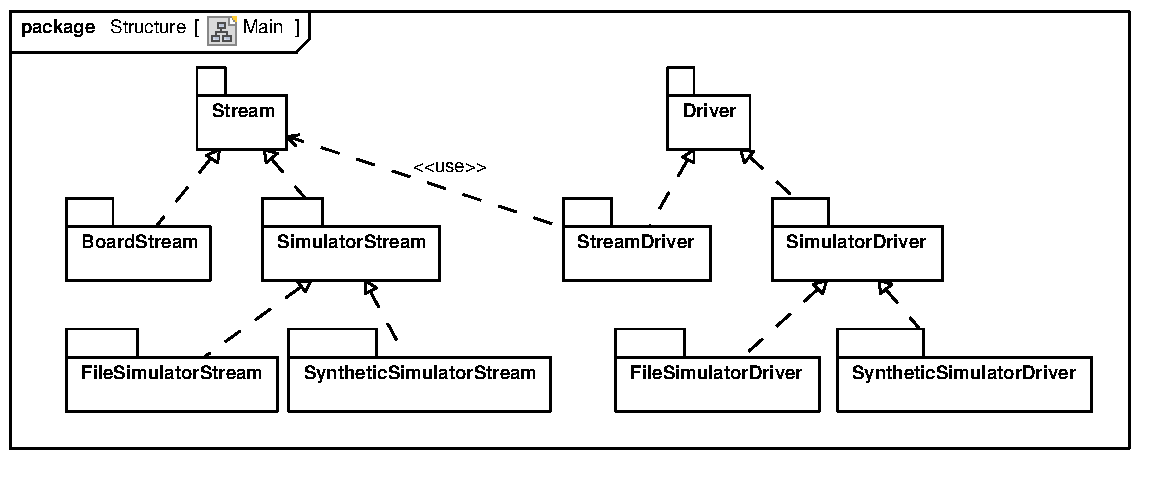
\includegraphics[scale=0.7]{UML_model/Class_Diagram__Structure__Main}
  \label{fig:class_diagram_main}
  \caption{Main packages class diagram.}
\end{figure}

The test package structure, which is shown in Figure
\ref{fig:class_diagram_test} reflects and mimics the code structure;
the tests for an abstract package are abstract, to be implemented by
the package that tests a corresponding system implementation; this is
a well known test pattern (the Abstract Test
Pattern\cite{thomas2004java}) used to test that the contracts are
respected in the implementations.  For instance, package \lil{DriverT}
contains abstract tests for the abstractions of package \lil{Driver},
package \lil{StreamDriverT} inherits the abstractions contained in
\lil{DriverT} and makes them concrete, to test the corresponding
implementation \lil{StreamDriver}; package \lil{StreamDriverT} also
contains stand alone tests written specifically for the implementation
contained in \lil{StreamDriver}.

\begin{figure}[htb!]
  \centering
  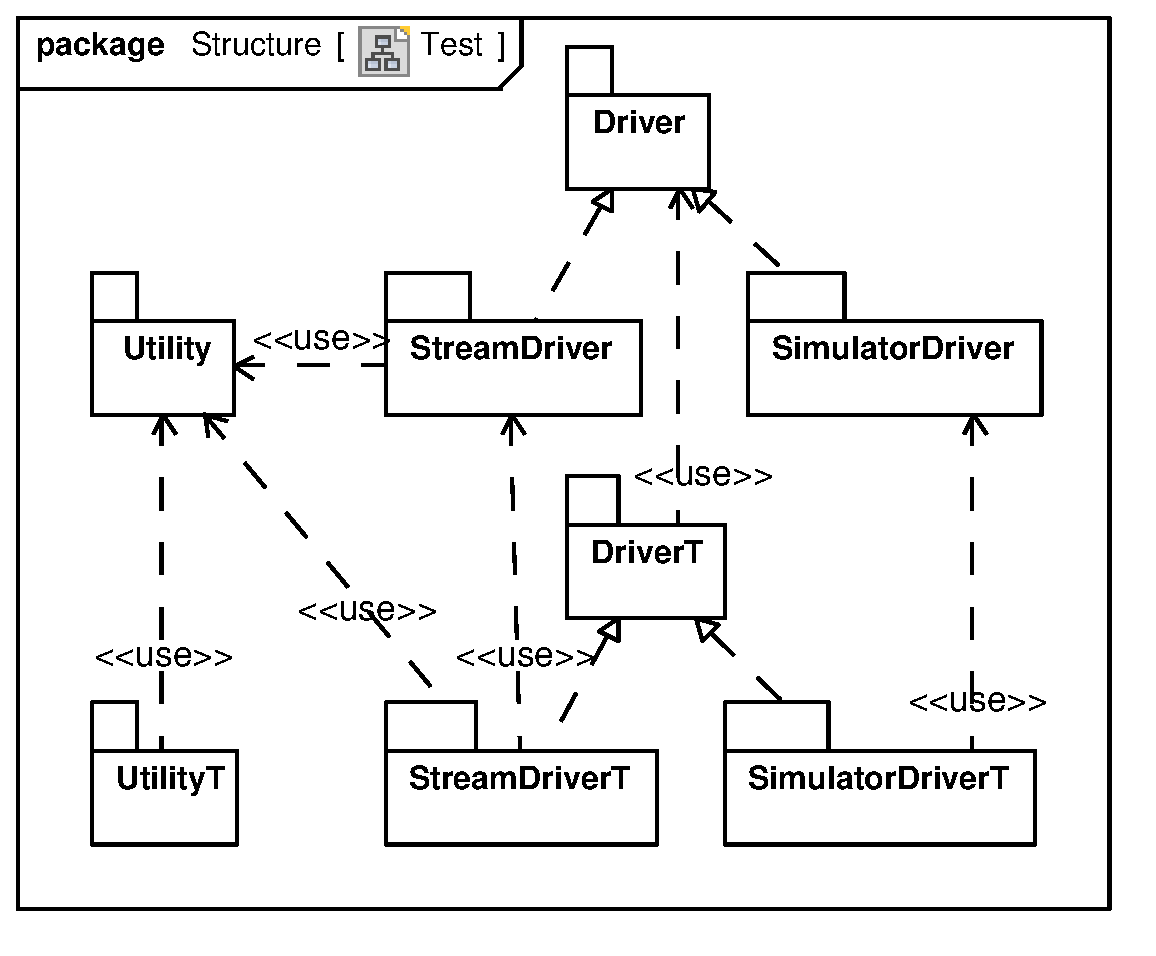
\includegraphics[scale=0.4]{UML_model/Class_Diagram__Structure__Test}
  \label{fig:class_diagram_test}
  \caption{Test packages class diagram.}
\end{figure}

\paragraph*{Generated tests}

The JML specification has been used to generate the tests.  A specific
tool of the JML2 suite is able to automatically generate
them\cite{Cheon-Leavens02}.

The test suite generated is a collection of fine grained unit tests.
For each public method a set of tests is generated.  The specified
behavior of the method is checked using the JML2 run time assertion
checker, hence, an oracle is not needed.  The generated tests send
messages to the method under test, once the initial precondition check is passed (if it is not passed, the test is discarded), the test catch assertion violation
exceptions;
if a precondition is not met the test is not run, if the
precondition is met the test is run and if the postcondition is not
met an exception is fired and the test fails.  The test data
used to build the tests is the only part that is required to be
provided by the user.

The resulting test package structure is shown in Figure
\ref{fig:class_diagram_generatedtest}.  The package dependencies are
defined by the specifications; for instance, \lil{SimulatorDriverST}
are generated tests, they test (hence use) the implementation
\lil{SimulatorDriver}, and have been generated using the
corresponding specification \lil{SimulatorDriverS}.  The
generated tests do not maintain the inheritance structure of the code
and the specification.

\begin{figure}[htb!]
  \centering
  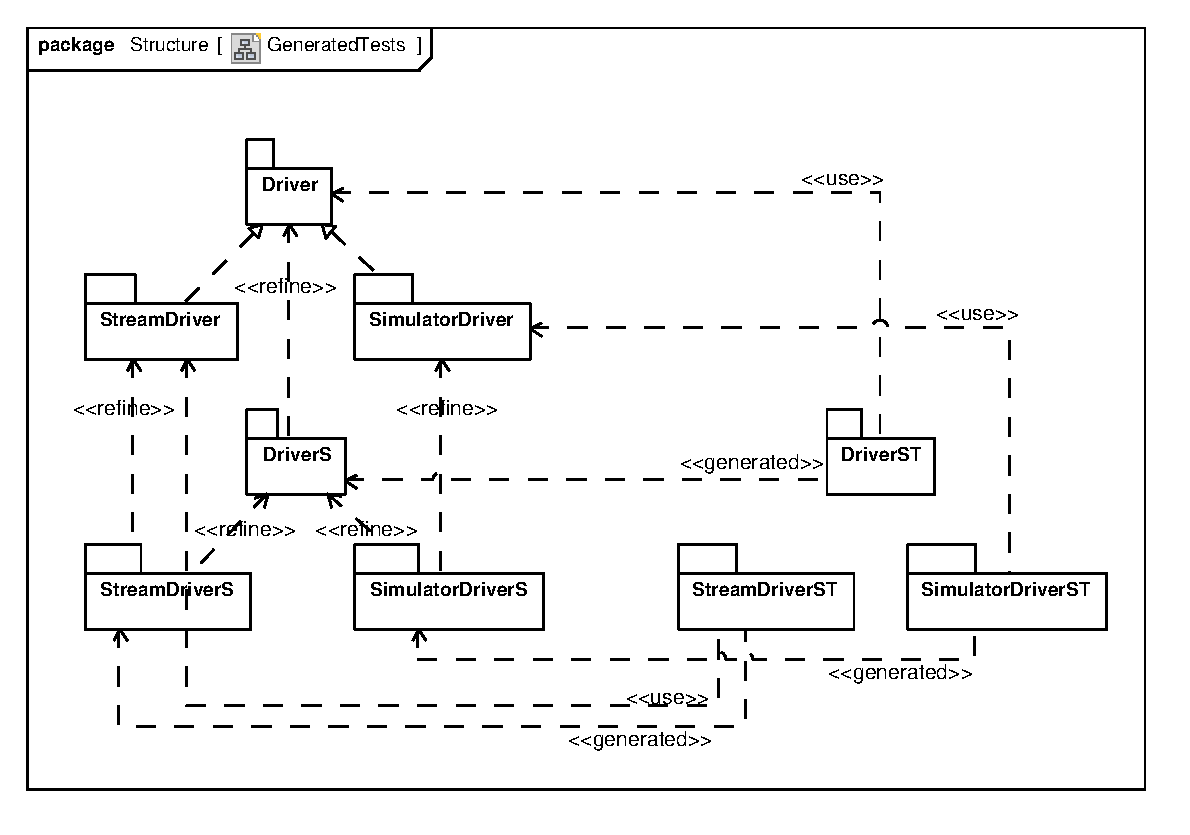
\includegraphics[scale=0.7]{UML_model/Class_Diagram__Structure__GeneratedTests}
  \label{fig:class_diagram_generatedtest}
  \caption{Generated test packages class diagram.}
\end{figure}

\paragraph*{On simulators, again}

A proper stub, driver and oracle should be identified for each method
under test to have proper unit test suite; stub, driver and oracle are
the usual components found in the harness that enable test
execution\cite{Binder1999}.  In
JUnit\footnote{\myhref{http://www.junit.org/}{JUnit}}, which is the
framework used to manage the implementation and execution of hand made
and generated unit tests, there is no clear distinction between
drivers, stubs, and oracles; none-less, even if a proper distinction
is not imposed by the framework, the conceptual distinction still
holds.

Hence, to properly unit test a package, we need:

\begin{description}
\item[Stub or Skeleton]: a piece of code that simulates the activity
  of the modules that are not under tests.
\item[Driver]: a piece of code that calls in a proper way the module
  under test.
\item[Oracle]: a mechanism used for determining whether a test has
  passed or failed, comparing the output of the module under test to
  the output the oracle determines the module should have.
\end{description}

Hand made unit tests and JML generated tests differ in how these
components are provided.  The distinctions and similarities are
summarized in Table \ref{tab:test_harness}.

\begin{table}[htbp]
  \caption{Hand made and generated tests harness.}
  \label{tab:test_harness}
  \begin{center}
    \begin{tabular}{|l|l|l|}\hline
      & \textbf{\textit{hand made}} & \textbf{\textit{JML}} \\\hline
      \textbf{\textit{Stub}} & to be provided & to be provided\\\hline
      \textbf{\textit{Driver}} & to be provided & automatic: 1 call\\\hline
      \textbf{\textit{Oracle}} & to be provided & 
      automatic: runtime assertion checker\\\hline
    \end{tabular}
  \end{center}
\end{table}

A module simulator can be used to ease the tasks of developing each
component of a test harness: it can be used as a stub, to simulate a
module needed by the module under test, it can be used as a driver, to
stimulate the module under test, it can be used as an oracle, if it
simulates the module under test.

In our system, the simulators has been used as stubs, so that we have,
during testing, a structure like the one shown in Figure
\ref{fig:class_diagram_streamdriver_test}.  In Figure
\ref{fig:class_diagram_streamdriver_test} the test suite
\lil{StreamDriverT} is using the \lil{SimulatorStream} to properly
simulate the \lil{Stream} used by \lil{StreamDriver}, which is the
system under test.

\begin{figure}[htb!]
  \centering
  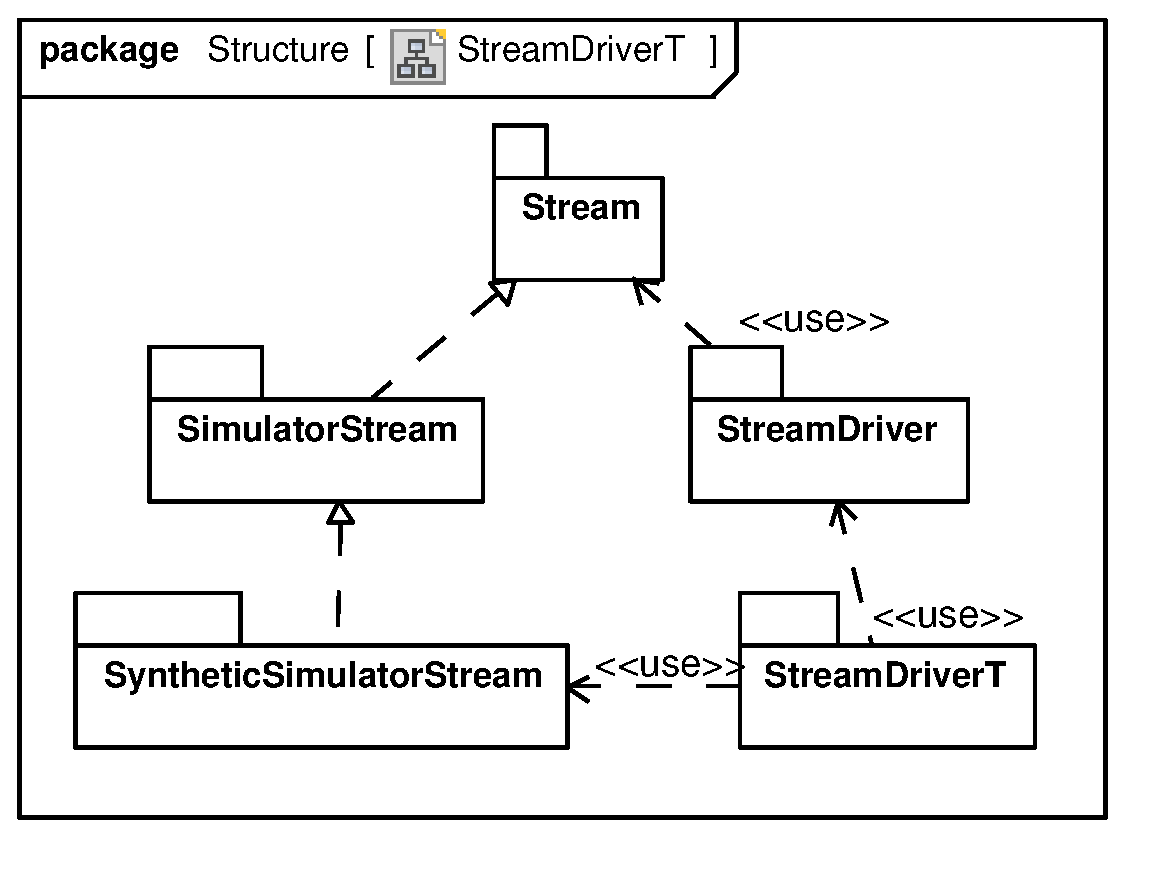
\includegraphics[scale=0.4]{UML_model/Class_Diagram__Structure__StreamDriverT}
  \label{fig:class_diagram_streamdriver_test}
  \caption{StreamDriver test packages class diagram: use of the stream
    simulator.}
\end{figure}

In our case, the use of simulators to enable unit testing, has been
essential to test the \STSB driver, since the physical board was not
available.  The simulators were have been used in both the hand made
and the generated test suite, since both of them need a proper set of
stubs to be executed.




% =====================================================================
\section{Test cases on the job}
\label{sec:test_cases_on_the_job}

JML specifications, the simulators, and both test suites has been used
to:

\begin{itemize}
\item verify hardware implementation;
\item verify driver implementation, with and without the physical
  board;
\item guide driver development.
\end{itemize}

The first \STSB prototype delivered was meant to build empty packets,
but the packets were built in a way not consistent with the
specification, the sentinel values used to delimit a packet were not
correct.  The board implementation errors were detected by simply
using the driver implementation, the \lil{StreamDriver} package.

The second prototype delivered was meant to build packets with values
taken from real sensors installed on the board.  The only sensors that
were not yet working were the sensors devoted to the fast rate data
streams, the audio sensors.  Only one error needed to be corrected in
the driver implementation, because of a (rare) combinations of
conditions that were not covered by the test cases, but that
occasionally showed up during real use.  One error have been
discovered in the low level system driver that the developed driver
was using (the system driver was outside of our development scope); to
eliminate the error an upgrade of the low level driver to a new
unreleased version was necessary.  No other errors were detected on
the driver side.

The second prototype respected the packet byte structure
specification, but was not fully compliant to the packet info
structure specification and the single packet rules.  The formal model
and the run time assertion checker enabled the detection of these
errors.  4 protocol errors regarding the packet info structure
specification, and 2 protocol errors regarding the single packet rules
has been found. No other errors, except the mentioned ones, have
been later on discovered.

The hand made test suite is composed by over 140 tests, while the
generated one is 100 times bigger, totaling over 14000 tests.  The big
number of generated tests (1 to 100 ratio), can be understood looking
closely at how the generated tests are created by the JML
framework. The generated tests are exploring the possible input
combinations on public methods, combining the type data ranges that
have been specified for the test suite (see \cite{Cheon-Leavens02} for
more details on how the JML framework works on generating unit
tests). For instance, let's suppose we want to test a method
\lil{m(int p1, int p2)} for a class \lil{C}; the data ranges specified
for type \lil{int} are \lil{\{1,2,3\}} and for type \lil{C} are the
instances \lil{\{c1,c2,c3,c4\}}. The JML framework generates $24 = 3
\times 3 \times 4$ tests, since they are the combination of the data
ranges involved (the data range of the parameters and the data range
of the type owning the method under test). Fortunately, not all the
generated tests are executed.

A generated test, as it was previously mentioned (see section
\ref{sec:test_cases}), is not executed, unless the preconditions of
the called method are satisfied. Thus, depending on the preconditions
specified for a method, the number of the generated tests that are
actually executed in the test suite can be significantly smaller 
compared to the total number of generated tests.

To compare in a quantitative way the effectiveness of the test suites,
code coverage metrics have been used; this is not the only measure
that have been considered, since it is almost unanimously accepted
that code coverage alone cannot asses the quality of a test
suite\cite{Marick1999,Chockler2006}.

Various coverage metrics exist, we analyzed the test suites with
statement code coverage (one of the simplest types)\footnote{The tool
  used to obtain statement code coverage metrics is
  \myhref{http://emma.sourceforge.net/}{Emma}.}: statement coverage
reports whether each executable statement has been encountered. This
code coverage metric is easy to implement, but lacks the capability to
explore the control flow graph associated to the code, that is,
decision branches are not explored. The coverage results are reported
in the Table \ref{tab:statement_code_coverage}.

\begin{table}[htbp]
  \caption{Statement code coverage result, categorized by source package.}
  \label{tab:statement_code_coverage}
  \begin{center}
    \begin{tabular}{|c|c|c|c|}\hline
      & \textbf{\textit{hand}} & \textbf{\textit{generated}} &
      \textbf{\textit{total}} \\\hline
      \textbf{\textit{Driver}} & $15.9 \%$ & $6.3 \%$ & $15.9 \%$ \\\hline
      \textbf{\textit{StreamDriver}} & $76 \%$ & $79.7 \%$ & $88.5 \%$ \\\hline
      \textbf{\textit{SimulatorDriver}} & $64.9 \%$ & $44.2 \%$ &
      $71.2 \%$ \\\hline
      \textbf{\textit{Utility}} & $98.1 \%$ & $74.5 \%$ & $98.1 \%$ \\\hline
    \end{tabular}
  \end{center}
\end{table}

Test suites execution time are very different, the hand made test suite, with the
run time assertion checking active runs completely in less than one
minute on an average PC, while the generated test suite runs in more
than 20 minutes (the rough ratio is $ 1 : 65 $). Most of the time is
spent on setting up the suite, only considering the real execution of
the tests, with no suite setup, the execution time reduces to less
than 4 minutes (the rough ratio is $ 1 : 10 $).



% =====================================================================
\section{Retrospective on test cases effectiveness}
\label{sec:test_cases_retrospectives}

The coverage measures reported in Table
\ref{tab:statement_code_coverage} are not high, in absolute
values. This is because of two different effects: non public methods,
and interfaces. The effect of non public methods (to be precise:
package Java visibility) is that these methods are taken into account
as well as public and protected ones during code coverage calculation;
but these methods are not part of the interface, they are not meant to
be called by the system, and they are only used in object
initialization or in object setups performed during unit tests. In
fact there are package and private code blocks that are not reachable
by construction from public and protected methods, and this is a
precise characteristic reflecting the code architecture, meant to ease
class instances setup and configuration for testing purposes. The used
statement coverage tool cannot be configured to distinguish these code
blocks, so this effect is unavoidable. The effect is mainly seen in
low \lil{SimulatorDriver} code coverage figures: the
\lil{SimulatorDriver} package has plenty of setup and initialization
non public methods.

Regarding interfaces, an interface contains no statements, so when an
interface method is called, it is the method of the implementation
class used that is actually covered. This effect is visible in
\lil{Driver} coverage figures: \lil{Driver} package contains
interfaces (that are not counted at all) and some very simple real
class (exceptions) that are not throughly tested. The net result is
extremely low statement code coverage figures because the very simple
classes are the only ones that are actually covered. This effect could
be easily avoided writing specific hand made tests for the simple
classes and including them in the classes for which tests are
generated.

The statement code coverage figures show that the test suites do a
good job on the most important package, that is, the
\lil{StreamDriver}. The generated test suite reaches almost $ 80 \% $,
while the hand made tests have only a slightly lower coverage ratio: $
76 \% $. But the combination of test suites is interesting, raising
the coverage ratio to $ 88.5 \% $. This is a clear indication that one
test suite is not completely overlapping the other: the test suites
are not to be considered alternatives, but they have to be used
together to achieve the higher benefits, they are complementary. This
consideration can be confirmed looking at the figures obtained for
\lil{SimulatorDriver} package as well.

The qualitative difference of the two test suites can be understood
analyzing how the suites are built. The hand made test suite primarily
focuses on small features and use cases fragments that the system must
implement, or for which an exceptional case has been specified. A test
case is to be considered a rough specification written in imperative
style. The common structure requires an object initialization,
followed by a hopefully not too long sequence of public methods taking
an object (or a set of objects) into a desired state; than the method
under test is called and the object state is finally inspected to
verify if it is in the expected state. Mock objects can be used to
limit the dependencies. The test suite should be composed only by unit
tests, but usually some tests are more complex to be called proper
unit tests; they can be seen as simple integration tests.

The generated test suite has a more focused and limited scope: since
only one method call is performed in each test, hence it is difficult
to explore complex behaviors. It is true that with a complete
specification, and specifying large enough data ranges (the
appropriate data ranges are combined to generate the tests), the
generated tests could theoretically achieve the same expressive power
as the hand made ones, but the price to pay would be expensive: much
longer and more complex specifications, requiring more time to be
designed and or updated, and more tests to be run, increasing the
already not so short computation time of the generated test suite.

The test suites gave their best when used in a combined approach: the
generated test suite, checking simpler behaviors, and the hand made,
checking the more complex ones.  During the development of the driver
code and the simulators, the generated test suite was helpful to test
the incrementally growing specifications and the finer details of each
method, while the hand made one was helpful to verify the behavior on
complex methods calls on objects initialized to specific
states. Having an hand made test suite also make the code style more
test oriented, which usually leads to a better quality and more
modularized source code\cite{Binder1999}.

The test suites has been used to verify different parts of the
systems, that is, the real system as well as the simulators.  The
multiple simulators and multiple test suites approach is not new,
since it has been often used in embedded systems software
testing\cite{Broekman2002}.  This is a general approach that can (and
should) be used to verify both the simulators built and the real
systems.  It can be easily implemented only if the code has been
structured following the already mentioned dependency inversion
principle\cite{martin1996dependency} (see Figure
\ref{fig:class_diagram_main}).

The combined test approach, driven by the packet protocol
specification, has been proved successful on verifying the protocol
itself and the software implementing it.  Nevertheless, it has to be
noted that the highest levels of the protocol are more problematic
(see \ref{sec:data_stream_and_protocol_description}: ``Packet sequence
rules'' and ``Packet input output asynchronous rules'').  On these
levels, the protocol properties regard sequences of packets, and
testing them can be tricky, since the sequences of packets are not
referred to explicitly, in the implementation.  Two possible
strategies can be used:
 
\begin{itemize}
\item Translate the packet sequence properties in local packet
  properties (when this is possible).  The advantage is to have
  properties shown as the usual pre-conditions, post-conditions and
  invariants.  However, the localized properties can be more complex
  and less intuitive and comprehensible than the original ones;
  finally, some of the global properties could prove themselves
  impossible to be translated into local ones.
\item Use separate utility classes, meant to verify a sequence of
  packages.  This approach is not clean, since it requires adding and
  using new classes, unneeded by the core implementation, to verify
  the protocol.  It has the advantage of keeping the properties that
  have to be verified mostly unchanged.
\end{itemize}

One problem we noticed regards the execution time of the generated
tests.  It is long for two reasons:

\begin{itemize}
\item Number of the tests generated. This problem is not directly
  addressable, since it is the heart of the test suite generation
  creation method itself: generating all the combinations of possible
  inputs for each method under test.
\item Runtime assertion checker. Each test is executed while RAC
  checks all the relevant properties. This problem, again, is not
  directly addressable. We can speculate that if the RAC assertions
  could be triggered on and off on single properties in a dynamic way
  (during runtime), a test suite would take advantage of this
  possibility, turning on the RAC only on the properties that have to
  be verified for the classes or methods under tests (and not for all
  the involved classes and methods); this could save time during the
  test suite execution.
\end{itemize}



% =====================================================================
\section{Related works}
\label{sec:related_works}

JML has been used previously to verify a communication protocol in
\cite{Hubbers2004}, but the protocol is a smart card protocol, and it
is well represented through state machines, which are then refined
into JML properties.  The approach is in waterfall style; than the
need to develop the protocol, the specification and the implementation
concurrently is not addressed.  No hand made or generated test suites
are used, the code is specified with JML assertions, refined by the
state machine specifications, and then checked statically with
ESC/Java2 static checker\cite{CokKiniry04} and at runtime with JML2
tools RAC\cite{BurdyEtal05-STTT}.

The JML-JUnit automatic test suite generation tool has not been widely
used or assessed. It is described by its own creators in
\cite{Cheon2002,Cheon2004,Cheon2005}; it has been used in
\cite{Oriat2004} and \cite{Cheon2005}, but only as a stand alone test
suite, and, more importantly, only against proof of concepts system,
it has never be proved against real complex systems.  A brief
assessment of the JML-JUnit tool has been made in \cite{Tan2004}, the
analysis is based on injecting random generated errors in the source
code, and then evaluating the ratio of the errors found by the test
suite: the results shows that the JML-JUnit tool is not effective
enough if used as a stand alone tool. No attempts on running or
evaluating the generated test suite alongside with an hand made test
suite are made.



% =====================================================================
\section{Conclusion}
\label{sec:conclusion}


\todo{specification and hand tests useful to drive, specification and
  hand tests and simulator useful to test, specification and generated
  tests useful for statement coverage and easy methods, specification
  useful to test hardware, hand useful to spec, spec useful to
  hand... test driven spec}


\section{Next papers}

\todo{remove and push this on a new paper}

\paragraph*{TDS: Test Driven Specification}

Approach:
\begin{itemize}
\item more specification used together: formal and not formal
\item formal specification is not complete: it is just good
  ``enough'', static checkers unfortunately cannot be used, since the
  specification is partial
\item use runtime assertion checker for formal specifications, on
  tests
\item use generated tests for formal specifications
\end{itemize}

Who drives what:
\begin{itemize}
\item specification (jml - formal specification or unit test -
  examples fragments) driven development
\item test driven specification
\item formal specification is not complete: it is just good
  ``enough'', static checkers unfortunately cannot be used, since the
  specification is partial
\item use runtime assertion checker for formal specifications, on
  tests
\item use generated tests for formal specifications
\end{itemize}

Benefits:
\begin{itemize}
\item real agile approach
\item real formal approach
\item use best of both worlds, do not try to use only on of them
\end{itemize}

Case example: actual paper, modified to fit the new parts, especially
the test driven specification part.

\paragraph*{BON}

\todo{describe approach: high level informal specifications with BON,
  iterative refinements of code, to distill test cases and formal
  specification of the interfaces}




% ======================================================================
%% \nocite{ex1,ex2}
\bibliographystyle{latex8} \bibliography{extra,%
  abbrev,%
  ads,%
  category,%
  complexity,%
  hypertext,%
  icsr,%
  knowledge,%
  languages,%
  linguistics,%
  meta,%
  metrics,%
  misc,%
  modeling,%
  modeltheory,%
  reuse,%
  rewriting,%
  softeng,%
  specification,%
  ssr,%
  technology,%
  theory,%
  web,%
  upcoming,%
  upcoming_conferences,%
  conferences,%
  workshops,%
  verification,%
  escjava,%
  jml,%
  nijmegen}

% ======================================================================
% Fin

\end{document}



%%% Local Variables: 
%%% mode: latex
%%% eval: 
%%% TeX-master: t
%%% End: 
